\documentclass[10pt,letterpaper]{article}
\usepackage[margin=0.65in]{geometry}
\usepackage[T1]{fontenc}
\usepackage{lmodern,booktabs,amsmath,microtype,xcolor,graphicx}
\usepackage[hidelinks]{hyperref}
\pagestyle{empty}
\setlength{\parindent}{0pt}
\setlength{\parskip}{5pt}
\begin{document}
{\Large\bfseries Exp 1: Ten Provers (Lean)}\hfill {\small Evaluation audit}
\vspace{2pt}\hrule
\textbf{Corrected conclusion.} The evaluation collapsed to compile-outcome reporting. Weights scored 0.996 from the first checkpoint, but a two-branch exit-code rule gives exactly the same predictions. This run does not establish the intended review-count crossover; the earlier conclusion is withdrawn.

\textbf{Design.} Ten Qwen3-8B workers per arm attempted small Lean list lemmas
with at most three compiler calls. The no-feedback, context, and LoRA arms each
ran 480 sessions over 4 rounds. DeepSeek-V3.1 reviewed
1440 reports. Context and weights received the same cumulative
no-feedback-arm reviews: context retrieved whole examples within 8,000 tokens;
rank-16 LoRA was retrained from base, with loss only on corrected final reports.
The scorer never supplied training targets or reward.

\textbf{Why the curve saturates.} The 120 traces (40 lemmas) contain 113 E4-only outcomes: 107 failed compiles and six sessions with no compile. Seven compile with \texttt{sorry}; one also has E6. There are \textbf{zero proved, partial, E1, E2, or E3 cases}. Always reporting E4 scores 0.942.
Each checkpoint produced five reports per frozen trace at temperature 0.7.
Score $P\times R$ is the product of precision and recall of the structured
header, not F1; prose is unscored. All four LoRAs emit identical headers on all 600 sampled reports: E4 after failure/no compile, E5 otherwise. Each misses the same E6 event, giving $(595 + 5/2)/600 = 0.99583$.

\begin{minipage}[t]{0.58\linewidth}
\vspace{0pt}
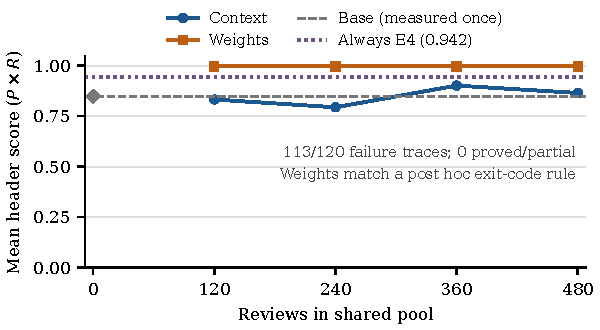
\includegraphics[width=\linewidth]{results-curve.pdf}
\end{minipage}\hfill
\begin{minipage}[t]{0.39\linewidth}
\vspace{3pt}\centering\small
\begin{tabular}{rccc}
\toprule
Pool & Base & Context & Weights\\
\midrule
0 & 0.848 & 0.848 & 0.848 \\
120 & 0.848 & 0.832 & 0.996 \\
240 & 0.848 & 0.793 & 0.996 \\
360 & 0.848 & 0.901 & 0.996 \\
480 & 0.848 & 0.864 & 0.996 \\
\bottomrule
\end{tabular}
\par\raggedright\footnotesize
Context actually receives 20--30 whole reviews per report under the 8,000-token cap. The x-axis counts available pool items, not visible examples.
Base is one reused measurement. No checkpoint was measured between 0 and 120 reviews.
\end{minipage}

{\small\textbf{Numerical result only.} At 480 reviews, weights minus context is 0.132 (paired 20-family bootstrap, 95\% CI [0.053, 0.227]).
The interval does not repair the missing outcome coverage.}

\textbf{Does Sun help the analyst?} A fresh DeepSeek-V3.1 analyst inspected
the same 120 sessions through transcripts (T), transcripts plus ordinary
Git history (T+), or transcripts plus Sun log/show/blame (S), with 15 calls per
episode and no access to earlier reviews or scorer verdicts. Sun recall was 0.583 versus 0.792 for transcripts, with similarly low precision. The primary E3/E6 comparison (overwrites or borrowed \texttt{sorry}) had only 1 inconsistency and is underpowered.
\begin{center}\small
\begin{tabular}{lrrrr}
\toprule
View & Precision & Recall & Specificity & E3/E6 recall\\
\midrule
Transcripts & 0.211 & 0.792 & 0.451 & 0.000 \\
Transcripts + Git & 0.230 & 0.667 & 0.683 & 0.000 \\
Transcripts + Sun & 0.220 & 0.583 & 0.622 & 0.000 \\
\bottomrule
\end{tabular}
\end{center}
{\footnotesize Budget-exhausted analyst episodes (T/T+/S): 0/0/2; scored as no flags.}

\textbf{Checks and limits.} Reviewer-corrected reports exactly matched the scorer in 90.6\% of sessions; 0 reviews failed.
An offline audit reproduced all 6,480 scores against saved compiler evidence and checked distinct adapter hashes, request identities, and raw outputs. The planned human smoke test has not been completed.
This is one live run with one LoRA seed per checkpoint. Parameterized lemma
families overlap across splits, and no self-label or shuffled-label training
controls were run. 384/480 corrected training reports omit prose, as do 580/600 final-checkpoint weights reports; the score does not penalize this.
The implementation checked pilot review completion, but had no gate for held-out
outcome coverage. A new calibrated run is needed for the intended comparison.

{\footnotesize\textbf{Reproducibility.} Sun was initialized for the experiment,
run, pilot, held-out and arm repositories. Saved compiler receipts, Sun commits,
review checks, samples, source hashes, and exported adapters support offline
recomputation. Including pilots, saved successful calls imply an uncached token cost of \$78.92; reservations total \$117.26, excluding storage. Neither is a provider invoice.\quad Run: \texttt{20260926-01}.}
\end{document}
